\documentclass[]{article}
%use European style
%\usepackage[a4paper,left=2cm,right=2cm,top=2cm,bottom=2cm]{geometry}

%few useful packages ------------------------------------------------------------------
\usepackage{setspace}
\let\Tiny=\tiny %remove annoying warnings
\usepackage[english]{babel}
\usepackage[latin1]{inputenc}
\usepackage{amsmath}
\usepackage{amssymb}
\usepackage{amsthm}
\usepackage{amsfonts}
\usepackage{colortbl}
\usepackage{xcolor}
\usepackage{eurosym}
\usepackage{enumitem}
\usepackage{chngpage}
\usepackage{fancyhdr}
\usepackage{fancyvrb}
\usepackage{float}
\usepackage{framed}
\usepackage{multirow}
\usepackage{graphicx}
\graphicspath{ {./images/} }
\usepackage{geometry}
\usepackage{lipsum}
\usepackage{tabularx}
\usepackage[linktocpage]{hyperref}

%define environment for code
\definecolor{orangepse}{RGB}{240,139,39}
\definecolor{redpse}{RGB}{222,6,61}
\newcommand{\rpse}[1]{\textcolor{redpse}{#1}}
\definecolor{dkgreen}{rgb}{0,0.6,0}
\definecolor{gray}{rgb}{0.5,0.5,0.5}
\definecolor{mauve}{rgb}{0.58,0,0.82}

\usepackage{listings}
\lstset{frame=tblr,
	language=R,
	aboveskip=5mm,
	belowskip=5mm,
	showstringspaces=false,
	columns=flexible,
	basicstyle={\small\ttfamily},
	numbers=none,
	numberstyle=\tiny\color{gray},
	keywordstyle=\color{blue},
	commentstyle=\color{dkgreen},
	stringstyle=\color{mauve},
	breaklines=true,
	breakatwhitespace=true,
	tabsize=3
}
%---------------------------------------------------------------------------------------


% New Commands ----------------------------
\newcommand{\bb}{\bigbreak\noindent}

\makeatletter
\renewcommand\section{\leftskip 0pt\@startsection {section}{1}{\z@}%
	{-3.5ex \@plus -1ex \@minus -.2ex}%
	{2.3ex \@plus.2ex}%
	{\normalfont\Large\bfseries}}

\renewcommand\subsection{\leftskip 4ex\@startsection{subsection}{2}{\z@}%
	{-3.25ex\@plus -1ex \@minus -.2ex}%
	{1.5ex \@plus .2ex}%
	{\normalfont\large\bfseries}}

\renewcommand\subsubsection{\leftskip 14ex\@startsection{subsubsection}{3}{\z@}%
	{-3.25ex\@plus -1ex \@minus -.2ex}%
	{1.5ex \@plus .2ex}%
	{\normalfont\large\bfseries}}
\makeatother


%opening
\title{Week 8:\\
	 \textit{``THE MACROECONOMIC EFFECTS OF GOVERNMENT
	 	ASSET PURCHASES: EVIDENCE FROM POSTWAR U.S.
	 	HOUSING CREDIT POLICY''}\\
	  by FIELDHOUSE et al.}
\author{Davide Davies-Biletta}

\begin{document}

\maketitle

\section{Introduction}
The authors seek to  investigate whether agency portfolio purchases of mortgage assets influence the availability and cost of housing credit and whether there are spillovers to other debt markets and economic activity more broadly.


\section{Method}

	\subsection{Issues with reverse causality}
	Agencies like Fannie Mae and Freddie Mac are forced to  systematically and rapidly respond to market conditions, such that changes in their mortgage purchasing activity reflect changes in housing credit demand and many other influences.
	\bb
	The correlation between their balance sheets and credit growth and mortgage rates are therefore likely to include elements of reverse causality. 
	
	\subsection{Narrative Analysis: A Solution}
	Narrative Analysis
	\begin{enumerate}
		\item Identify historical policy changes leading to expansions or contractions in agency mortgage holdings
		\item Measure their relation to short-run credit or cyclical shocks
		\item Measure impact of mortgage purchases by agencies.
	\end{enumerate}
	Credit policy changes are often reactions to cyclical conditions in mortgage and housing markets, the recent crisis being a prime example. However, many interventions are motivated by other longer-run objectives, such as increasing home ownership. 
	\bb
	Based on an extensive analysis of historical sources the authours classify each significant policy change
	\begin{itemize}[leftmargin=10ex]
		\item Cyclical Considerations
		\item Non-cyclical Considerations
	\end{itemize}
	Non-Cyclical events are used as an instrumental variable in regressions of a variety of outcome variables on measures of agency purchasing activity.
	\bb
	Agency purchasing effects credit in markets with pervasive market frictions providing credit to residential buyers. This leads to increased activity in refinancing operations, and increased originations. This is followed by a temporary reduction in the mortgage rate.
	\bb
	Agency purchases also affect prices in other asset markets.
	
	\bb
	Their approach permits an analysis beyond the very short-run response of financial variables, and unlike the cross-sectional studies, provides direct evidence on aggregate rather than relative effects.
	
		 \subsubsection{Steps to creating an Narrative Approach Instrumental Variable}
		 \begin{enumerate}[leftmargin=15ex]
		 	\item Identifying significant policy changes affecting agency portfolios
		 	\begin{itemize}
		 		\item Long list of sources
		 	\end{itemize}
		 	\item Quantifying their ex ante projected impact on agency holdings
		 	\item Pinpointing the timing of when the policies became publicly known
		 	\item Classifying each policy change as either cyclically or non-cyclically motivated
		 	\item Restricting the sample for consistent use as an instrument for agency purchasing activity.
		 \end{enumerate}
	
	\subsection{Quantitative Analysis}
	Jord� (2005) Local Projections method by two-stage least squares (2SLS).
	
	\begin{itemize}[leftmargin=10ex]
		\item First Stage:\\
		Make sure the noncyclical policies lead to more agency mortgage purchases
		\begin{itemize}
			\item This checks the validity of the instrument.
		\end{itemize}
		
		
		\item Second Stage:\\
		Test weather these purchases have effects on the market.
	\end{itemize}
	
	\section{Data}
	The Authors use a large and varied set of sources to construct their narrative approach.
	
	\bb
	The monthly sample contains 45 months with interventions in the post-1967 sample (there are 52 interventions in total,
	but some occur within the same month). Out of these, 28 are classified as cyclically motivated, leaving 19 distinct noncyclically motivated policy events. In the sample that excludes interventions after December 2006, there are 15 cyclically and 17 noncyclically motivated policy events after monthly aggregation
	
	\begin{center}
		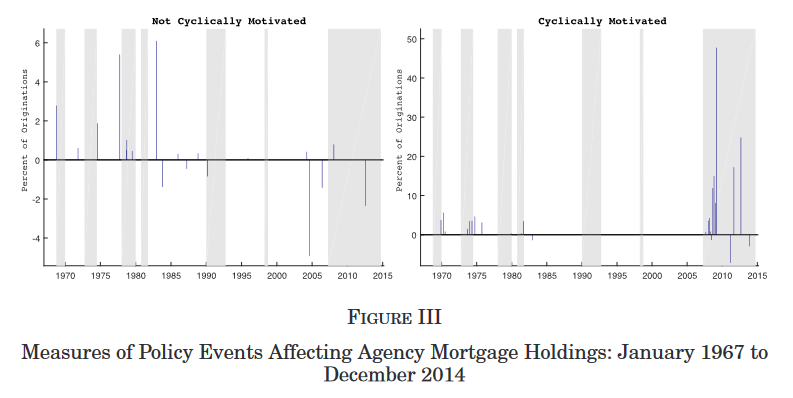
\includegraphics[width=\textwidth]{screenshot001}
	\end{center}
	
	\section{Results}
	Estimates indicate that each additional \$1 in agency mortgage purchases leads to a \$3 to \$4 cumulative in-
	crease in mortgage originations over the course of three to four years, and a net expansion in the stock of mortgage debt of around \$1.
	\bb
	The expansionary effects on housing credit are accompanied by temporary reductions in mortgage interest rates, which fall by 10 to 15 basis points for more than a year following an increase in agency purchases of 1\% of trend originations.
	\bb
	\subsection{Other markets}
	\begin{itemize}[leftmargin=10ex]
		\item Positive impact on housing starts and homeownership
		\item Increase house prices
		\item Stimulate private sector consumption
		\item No effect on unemployment or personal income
	\end{itemize}
	

\section{Criticism }
While the paper is well constructed to defend itself from questions of endogeneity,
How generalisable is this information? Is this likely to work in countries where housing prices are higher, and long-term renting is more common.

\bb
How valid really are the instruments? 

\end{document}
